

\newpage
\section*{Introduction}
\noindent
Maintenance of structures is considered as a set of practices performed to ensure that the structure fulfills its duties and provides an adequate level of safety and serviceability during 
its service life. A proper maintenance planning can prevent unexpected failures to happen on a structure. Therefore, it can be seen as a tool to ensure the return of investment for the 
owners of structures after an expected period of time. One should keep it in mind that the maintenance cost of civil structures (e.g. bridges, wind turbines, power plants, railways, etc.) 
is relatively high. Hence, the maintenance optimization of civil structures has gained more attention during the past decades since the number of aging structures is increasing while the 
budget for the maintenance is limited. 


To understand well the importance of the maintenance planning for a given structure let's say a bridge, one can study the consequences of different failures on the structure. In the small
level, failures on the bridges can cause stopping the traffic for carrying out the emergency repair actions. This can bring loss of capital and reputation for the bridge owner in one hand 
and wasting the time and inconvenience for the drivers. However, in the bigger scale, the failure can lead to catastrophic damages including collapse of the structure, loss of lives, 
and environmental and social damages. Therefore, a proper maintenance planning is very crucial for the owners of structures since it can prevent the future unexpected adverse events to 
occur on the structure. 


Before preparing a maintenance strategy for structures, it is important to identify the failure modes of structures since each mode might need a particular maintenance actions to be able 
to remove or lessen the cause of failure. Statistical information form the past failures of metallic structures show that the most frequent failure mode respectively are: scour of
pies/foundations, buckling, fatigue, impact, and fracture. Although, scour is an important failure mode for all bridges, fatigue and fracture taken in combinations appear to be the most 
critical failure mode for metallic bridges. It is obvious that a proper maintenance planning should involve different actions to mitigate the failure occurrence by any failure mode. 
However, failure modes that are more likely to happen will take higher attention within the maintenance framework. Therefore, one can say that maintenance against fatigue and fracture 
has the priority in metallic structure that work under cyclic loading. 


Fatigue is one of the main degradation processes on metallic structures that are working under cyclic loading (e.g. traffic and environmental loading). Fatigue process can start with the 
crack initiation which can be caused by many drivers such as material imperfection, cyclic loading, local stress concentration, corrosion, etc. The initial crack will propagate under cyclic
loading even if the resulting stress range on the crack region is less than the yielding stress of the material. This can deteriorate the structure and causes failure if the crack has not 
been detected before reaching its critical length. The crack length remains very small for a major part of the fatigue life of a structure and the crack propagation time from a detectable 
crack length to a critical length that causes failure is relatively short compared to the fatigue life. Therefore, it is really challenging to detect a fatigue crack before it puts the 
structure through a tragic failures. Another challenge in fatigue process is that accurately predicting the fatigue failure is difficult since it is associated with huge level of uncertainty. 
The uncertainty is related to different factors which are influencing the fatigue resistance such as fatigue loading, stress calculation, material properties, fatigue resistance data, fatigue 
accumulation crack growth model, weld geometry, etc. \ac{SHM} is a good practice that helps to reduce the uncertainty involved in fatigue resistance calculations. 


One important factor that makes the existing structures different than the newly constructed ones is that they have already experienced the real life loading conditions. \ac{SHM} can be
employed on existing structures to evaluate the state of the entire structure. \ac{SHM} is a process focusing on observing, measuring, recording, and processing of the actual data related to the 
structure in real time. It provides valuable information about the current status of a structure for the owners of the structures and decision makers. This information can be used to update
the performance indicators (reliability and risk) or lifetime distributions (availability and hazard) for a given structure to perform a better maintenance planning. For instance, a 
reliability-based maintenance tries to keep the reliability level of the structure higher than a given threshold without considering the consequences of the failure. However, a risk-based
maintenance take them into the consideration. 


Considering the maintenance against fatigue, time-dependent reliability index can provide a good indicator for decision makers. The reason for choosing this indicator is that fatigue is a
degradation process involving stochastic loadings and random inputs in one hand. In the other hand, a time-dependent indicator provides a better criterion for decision making process since 
one can estimate when in time the failure will happen. Performing the time-dependent reliability analysis is basically different than time-independent one since the objective is to find the 
cumulative failure probability for a given period of time. Therefore, finding this failure probability is quiet challenging for problems with non-monotonic and computationally expensive 
performance functions. As said before, monitoring information can be used to have an updated indicator for a better maintenance optimization. 


The indicator chosen from the performance indicators or lifetime distributions can be employed as a decision variable for the optimization of the maintenance allocation. In general, 
minimizing the cost is the main objective of the optimal maintenance planning. Therefore the optimization model tries to search among available maintenance actions and intervention 
times throughout the structural service life to find the solutions with minimum costs of maintenance within the feasible domain which is defined by predetermined constraints (e.g. time 
between interventions, reliability threshold, maintenance types and actions, etc.). Preparing an appropriate cost model and constraints for the optimization is a very important task in 
this step. 


According to what has been discussed shortly, it can easily be realized that improving methods and strategies in optimal maintenance planning of civil structures is a very complicated task since it
covers a very big range of topics and involves many challenges coming from different sources. Therefore, to improve the current practices in structural maintenance planning it is 
necessary to address the available challenges within the topics explained before such as application of \ac{SHM}, degradation models, time-dependent risk and reliability methods, optimization
models, consequence modeling, etc. In the next part, the objectives and contributions of this research towards optimal maintenance planning of structures is described. 



\section*{Objective and scope of the research}

\noindent
The overall goal of this study is to address some of the current challenges available in the domain of optimal maintenance planning of existing structures against fatigue with the help of 
\ac{SHM} data. Considering a reliability-based maintenance optimization our objective is to address challenges related to a: fatigue reliability assessment, b: application of monitoring 
information, and c: allocation and optimization of maintenance strategies. Addressing these challenges can define different steps of this study. Figure \ref{fig:phases} shows how different 
steps can be connected to each other in order to perform maintenance planning against fatigue by using monitoring data. 

\begin{figure*}[ht]
\centering
  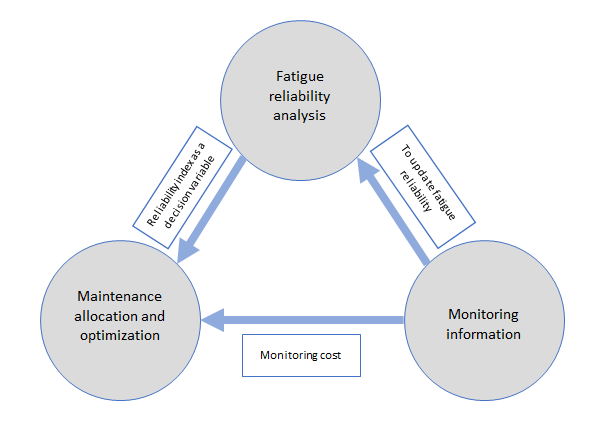
\includegraphics[width=0.75\linewidth]{figures/steps_flow.png}
  \caption{Main phases of maintenance planning against fatigue}
  \label{fig:phases}
\end{figure*}


Within the first step, fracture mechanism and S-N curves are two regular approaches that are used to evaluate fatigue damage and provide a proper limit state for fatigue reliability analysis. 
Employing fracture mechanism approach is depending on if inspections show a crack development in the structure, while S-N curve approach is based on experimental data which provides an estimation 
of number of cycles to fail. Performing the fatigue reliability analysis under a time-dependent framework seems more reasonable since it is a degradation process working under stochastic
loading that is highly dependent on time. The challenge in time-dependent reliability analysis is related to the problems involving computationally expensive and non-monotonic performance 
functions. Hence, we have developed an efficient methodology to perform time-dependent reliability analysis that is called AK-SYS-T. This methodology uses the similarity between system 
reliability and time-dependent reliability in a way to apply efficient system reliability methods for time-dependent problems. In this approach, Kriging meta-modeling is used to replace the 
computationally expensive performance functions. The learning process in AK-SYS method helps to enrich the Kriging meta-models very efficiently without needing to an optimization process.
The results show that AK-SYS-T can compete well in terms of efficiency and accuracy with the state of the art methods.


The second step is related to how to get benefit from monitoring information. \ac{SHM} provides us with valuable information about the current situation of civil structures. 
Advances in data acquisition, inspection technologies, and data management accompanied with the effective integration of \ac{SHM} into an intelligent system can help to improve the current practices 
on structural maintenance and management. Fatigue phenomenon is a function of some random and uncertain parameters such as loading, material properties, crack parameters, etc. Therefore, 
utilization of \ac{SHM} into structural fatigue life assessment can be a great help to reduce uncertainties toward fatigue life analysis. It also helps decision makers to find the best solution to 
prevent fatigue failures to increase the structural lifetime. The challenge here is related to the way of employing the information coming from monitoring data. 


Depending on the type of monitoring data, classical statistics or Bayesian inference can be used. In case of having adequate monitoring data, classical statistics is preferred. However, if the 
data in not sufficient, prior information about the phenomenon in a Bayesian inference framework will be employed to provide more informative results. With this respect and using the classical 
statistics, a study has been developed on long-term monitoring data available at \ac{EPFL} on Chillion viaduct. Seasonal ARIMA which is a method to study 
time series is used to prepare a loading model for long-term monitoring data on transversal rebars in the concrete deck of the bridge. The aim is to capture seasonality effect in traffic 
loading and to provide a model that gives more detail about structural fatigue loading. This load model can be used within S-N approach or fracture mechanism with some adjustments.


In the last step, a study has been developed to study the crack propagation in the deck plates of the orthotropic decks under transversal tension. The crack can be initiated in the root of 
the fillet weld where the stiffener is welded to the deck plate. Propagation of the crack in this area towards the deck plate is very crucial because this kind of cracks are very difficult 
to inspect and detect while the crack length can reach the critical threshold without being noticed. Transversal tension in the deck plate can be considered as a main reason for this kind of 
propagation. Therefore, the goal here is to study how the transversal tension can influence the direction of the crack propagation. The transversal tension in the deck plate can be caused 
by traffic loads, residual stresses, and weight of the structure (for the bridges with a long cantilever arm). To conduct this study, \ac{X-FEM} implemented in Code-Aster developed by \ac{EDF} 
is used to perform crack propagation analysis, and for the crack initiation a simple \ac{FEM} combined with cumulative fatigue damage under cyclic loading is used. Another objective of this step 
is to study some maintenance strategies to prevent the crack propagation through the deck plates. Therefore we study the effect of welding some horizontal plates in the middle of stiffeners 
to connect stiffeners to each other to add some toughness to the structure. 


As it was previously mentioned, the goal of this study is to add some contributions to optimal maintenance planning of existing structures. These contributions can help to improve the 
maintenance planning of structures by providing new methods and approaches to the topic which are going to be described with details in the following sections. 



\section*{INFRASTAR, its objectives, and challenges to accomplish the PhD} 

\noindent
INFRASTAR stands for "Innovation and Networking for Fatigue and Reliability Analysis of Structures - Training for Assessment of Risk". It has received funding from the European Union’s 
Horizon 2020 research and innovation program under the Marie Skłodowska-Curie actions. INFRASTAR involves twelve \ac{ESR} working in different research institutes, 
universities, and companies in five European countries (France, Germany, Switzerland, Denmark, and Poland). The host company for this PhD is PHIMECA Engineering in France in cooperation 
with Université Clermont Auvergne. 

The main goal of INFRASTAR is to improve the knowledge, skills, expertise, and to propose innovative solutions toward optimal maintenance and management of civil structures against fatigue
(particularly for bridges and wind turbines). Three major challenges are trying to be addressed within this program: 1) advanced modeling of concrete fatigue behavior, 2) new non-destructive 
testing methods for early aged damage detection, and 3) probabilistic approach of structure reliability under fatigue. With this respect three work packages can be recognized where four ESRs
are working under each work package. Work package one is related to "monitoring and auscultation". The second work package deals with "structure and action models", and the third one covers 
"reliability-based approaches for decision making". 

To achieve this goal, a cross-experience and inter-disciplinary cooperation between ESRs within different research centers is necessary. For this reason different secondments in addition to 
training weeks are considered for each ESR to visit the other research centers within the program to be able to collaborate with other ESRs and research centers. For instance, two secondments 
(each one three month long) was considered for this project. The first secondment took place at \ac{EPFL}, department of civil engineering and the second one was carried out at IFSTTAR
and Cerema. Also, three training weeks was completed during this PhD in BAM Berlin, EPFL, and University of Aalborg respectively. 

Providing a framework in which each ESR has to collaborate with other ESRs and researchers in different working environments rather than staying in the host institute is an excellent 
opportunity for them to improve their scientific, networking, and communication skills. However, one can face different difficulties mostly concerned with secondments since they take a big 
portion of the PhD time which in total is about three years. To enumerate some of those difficulties one can mention the travel issues, relocating to a new city or country, integrating to 
new work places, and the most important one which is developing new research topics that makes a relation between the thesis subject and in the same time falls within the research interests 
of the hosting institute during the secondment. 

To put it in a nutshell, the topics that are developed during this PhD are tried to be chosen in way that are, in one hand, related to the main topic of the thesis which is "Optimal 
maintenance planning of existing structures using monitoring data" to keep the consistency among the topics of the thesis. In the other hand, since some of the topics have been developed 
during the secondments, it has been tried to keep the hosting research centers happy and perform a study that is interesting for them also. Hence, the topic of the thesis is updated to 
"Towards optimal maintenance planning of existing structures using monitoring data". 

\section*{Summary}

\noindent
According to what has been described before, four chapters have been considered for this thesis. Chapter 1 is devoted to the practices on structural maintenance planning. In this chapter
it is tried to have a review on maintenance actions and indicators, structural deterioration, maintenance optimization and application of SHM for maintenance planning. The second chapter
is related to time-dependent reliability analysis. The new methodology to address time-dependent problems is introduced in this chapter supported by some examples form the literature to 
validate the algorithm. In chapter 3, the crack propagation in orthotropic deck plates is studied. It is shown that the root of the fillet weld (connecting the stiffener to the deck plate)
is a critical point and the crack can initiate from this area. X-FEM is used to perform the crack propagation under different tension levels in the deck plate to evaluate the direction of
crack propagation. Finally, some applicational examples are provided in chapter 4 to connect different steps of the study. For example in one example it is tried to employ AK-SYS-T on a crack 
propagation case to show the efficiency and the accuracy of the method on fatigue problems. It should be noted here that the study that has been developed on "Application of time series
methods on long-term structural monitoring data" has not been introduced in a chapter but the related paper is provided in the appendix since this work has not been done under the supervision 
of my thesis supervisors but under the supervision of professor Eugen Brühwiler at EPFL.























